\documentclass[12pt,a4paper]{article}

% ============================================================
% PACKAGES
% ============================================================

\usepackage[utf8]{inputenc}
\usepackage[T1]{fontenc}
\usepackage{geometry}
\usepackage{graphicx}
\usepackage{booktabs}
\usepackage{array}
\usepackage{longtable}
\usepackage{float}
\usepackage{xcolor}
\usepackage{enumitem}
\usepackage{fancyhdr}
\usepackage{setspace}
\usepackage{titlesec}
\usepackage{hyperref}
\usepackage{tikz}

\usetikzlibrary{
    positioning,
    arrows.meta,
    shapes.geometric,
    fit
}

% ============================================================
% PAGE SETUP
% ============================================================

\geometry{
    top=1in,
    bottom=1in,
    left=1in,
    right=1in
}

\onehalfspacing

% ============================================================
% HEADER / FOOTER
% ============================================================

\pagestyle{fancy}
\fancyhf{}
\fancyhead[L]{HR Process Digital Twin}
\fancyfoot[C]{\thepage}

% ============================================================
% HYPERLINKS
% ============================================================

\hypersetup{
    colorlinks=true,
    linkcolor=black,
    citecolor=black,
    urlcolor=blue
}

% ============================================================
% DOCUMENT
% ============================================================

\begin{document}

% ============================================================
% TITLE PAGE
% ============================================================

\begin{titlepage}

\begin{center}

\vspace*{1cm}

{\Large \textbf{SYNOPSIS}}

\vspace{1.5cm}

{\LARGE
\textbf{DESIGN AND DEVELOPMENT OF AN}\\
\vspace{0.3cm}
\textbf{ HUMAN RESOURCE MANAGEMENT SYSTEM}\\
\vspace{0.3cm}
\textbf{USING A PROCESS DIGITAL TWIN APPROACH}
}

\vspace{2cm}

{\large
A Project Synopsis
}

\vspace{1.5cm}

Submitted by

\vspace{0.5cm}

\textbf{\underline{\hspace{7cm}}}

\vspace{0.7cm}

Under the Guidance of

\vspace{0.5cm}

\textbf{\underline{\hspace{7cm}}}

\vfill

\textbf{}

\vspace{0.4cm}

\textbf{\underline{\hspace{7cm}}}

\vspace{0.4cm}

\textbf{2026}

\end{center}

\end{titlepage}

% ============================================================
% ABSTRACT
% ============================================================

\section*{Abstract}

The proposed project aims to design and develop an Human
Resource Management System (HRMS) using a Process Digital Twin
approach. The system goes beyond conventional HR record management
by maintaining a live digital representation of human-resource
processes, their current states, participating users, approvals,
events, and historical changes.

The proposed HRMS covers the major processes required for
employee and HR operations. These include authentication and user
management, role-based access control, employee management,
employee onboarding, job requisition and manpower planning, job
opening and vacancy management, attendance, leave, payroll and
statutory compliance, performance management, employee benefits,
Employee Self-Service, internal promotion, internal transfer,
resignation and exit management, document management, company
asset management, and a configurable application/request engine.

The Process Digital Twin represents HR activities as stateful
processes. For example, employee onboarding progresses through
selection, onboarding, document verification, employee creation,
account creation, and active employment. Similarly, resignation
progresses through submission, manager review, HR approval, exiting,
and exit. Important state changes are recorded as events and
preserved as historical records instead of overwriting previous
information.

A reusable Workflow Engine is provided for configurable,
multi-step approvals. Different request types can have different
approval chains, and approvers such as the employee's current
manager, new manager, or authorized HR users are resolved
dynamically.

The platform also contains a Dynamic Module Engine and Dependency
Engine. Authorized developers can register future modules by
defining their metadata, permissions, workflows, and dependencies.
The Dependency Engine validates whether required modules exist,
are active, and free from circular dependencies
before activation.

The proposed system follows a modular monolith architecture and is
designed to run locally using free and open-source technologies.
React.js, Vite, and Vanilla CSS are used for the frontend,
while Node.js, Express.js, and pg (node-postgres) are used
for the backend. PostgreSQL is used as the primary database,
providing a robust, persistent storage solution.

% ============================================================
% TABLE OF CONTENTS
% ============================================================

\newpage

\tableofcontents

\newpage

% ============================================================
% 1. INTRODUCTION
% ============================================================

\section{Introduction to Digital Twin}

A Digital Twin is a digital representation of a real-world entity, process, or system that maintains a continuous or controlled connection with its real-world counterpart through data, enabling its state, behavior, and lifecycle to be represented and monitored digitally. In industrial practice, Digital Twins are used to improve visibility, traceability, analysis, decision-making, and process optimization across the lifecycle of an entity.

Digital Twins can represent different levels of scope, including components, assets, processes, and systems. A Process Digital Twin specifically focuses on representing the sequence of activities, participants, states, decisions, and outcomes involved in a process. It can also support controlled simulation of process behaviour by evaluating defined states, transitions, events, and dependencies.

\subsection{Basic Concept}

A Digital Twin generally consists of:

\begin{enumerate}
    \item \textbf{Real Entity or Process:} The actual object,
    activity, or process being represented.

    \item \textbf{Digital Representation:} A software
    representation containing information about the entity or
    process.

    \item \textbf{State and Event Information:} Information
    describing the current state and the events that caused changes
    in that state.
\end{enumerate}

The Digital Twin therefore provides a continuously maintained
digital view of the entity or process.

\subsection{Digital Twin and Process Management}

When applied to a process, the Digital Twin represents the complete
flow of activities rather than only storing the final result.

A process may contain:

\begin{center}
\textbf{Input}
$\rightarrow$
\textbf{Activity}
$\rightarrow$
\textbf{Review}
$\rightarrow$
\textbf{Approval}
$\rightarrow$
\textbf{Decision}
$\rightarrow$
\textbf{Outcome}
\end{center}

The current state of the process and its historical events can be
maintained in the Digital Twin.

% ============================================================
% 2. TYPES OF DIGITAL TWINS
% ============================================================

\section{Types of Digital Twins}

Digital Twins can be classified according to the level of the
entity or process being represented. The major types are Component
Twin, Asset Twin, Process Twin, and System Twin.

\subsection{Component Digital Twin}

A Component Digital Twin represents an individual component or sub-component of a larger industrial product, machine, or production system. It focuses on the characteristics, condition, operational state, and relevant lifecycle information of that specific component.

In an IFB air-conditioner manufacturing plant, a Component Digital Twin can represent an individual AC component such as a compressor, condenser coil, evaporator coil, fan motor, or motor bracket. For example, a digital representation of a compressor can maintain information such as its identification, specification, production status, inspection results, quality status, and maintenance or lifecycle information.

Thus, a Component Digital Twin provides a digital representation of an individual component, which can subsequently be associated with the larger AC unit, manufacturing process, or production system.

\begin{itemize}
    \item Temperature
    \item Vibration
    \item Wear
    \item Operating condition
    \item Health status
\end{itemize}

The Component Twin provides a detailed digital representation of
one individual component.

\subsection{Asset Digital Twin}

An Asset Digital Twin represents a complete individual asset that consists of multiple components and performs a specific function within an industrial environment. It maintains relevant information about the asset's configuration, operational condition, performance, maintenance, and lifecycle.

In an IFB air-conditioner manufacturing plant, an Asset Digital Twin can represent an individual production machine or equipment such as a stamping machine, brazing machine, coil-processing machine, testing machine, or other dedicated manufacturing equipment. For example, a digital twin of a stamping machine can maintain information such as its machine identification, specifications, operating status, production activities, maintenance history, inspection information, and associated production records.

Thus, an Asset Digital Twin provides a digital representation of a complete industrial asset, allowing its condition, usage, maintenance, and lifecycle to be monitored and managed digitally.

\subsection{Process Digital Twin}

A Process Digital Twin represents a complete process consisting of interconnected activities, operations, resources, participants, inputs, outputs, and process states. It digitally represents how a process operates and how its state changes throughout its lifecycle.

In an IFB air-conditioner manufacturing organization, different organizational and operational processes are supported through systems such as Human Resource Management System (HRMS), Customer Relationship/Customer Request Management (CRN), and Enterprise Resource Planning (ERP). These systems involve interconnected processes, activities, users, data, approvals, and state transitions.

For example, the HRMS manages processes such as employee onboarding, leave approval, performance evaluation, internal promotion, internal transfer, and resignation. The ERP supports organizational processes related to planning, materials, inventory, procurement, production, and other enterprise operations, while the CRN supports customer-related processes and interactions.

A Process Digital Twin can therefore represent the flow of these processes, including their activities, dependencies, responsible users, current states, and historical events

\subsection{System Digital Twin}

A System Digital Twin represents an entire interconnected system consisting of multiple processes, assets, resources, and subsystems that work together to achieve a common objective. It focuses on the overall operation of the system and the relationships and interactions between its different processes and components.

In an IFB air-conditioner manufacturing plant, a System Digital Twin can represent the complete manufacturing procedure, covering different production areas such as stamping shop, coil shop, paint shop, assembly, testing, and final goods. It can digitally represent how materials and components move between these stages and how the different processes interact to produce the final air-conditioning unit.


% ============================================================
% 3. SELECTION OF PROCESS DIGITAL TWIN FOR HR
% ============================================================

\section{Selection of Process Digital Twin for HR}

The proposed project selects a \textbf{Process Digital Twin} for
representing Human Resource processes.

Examples of these processes include:

\begin{itemize}
    \item Employee onboarding
    \item Leave application and approval
    \item Employee loan application
    \item Special allowance application
    \item Performance evaluation
    \item Internal promotion
    \item Internal transfer
    \item Job requisition
    \item Resignation and exit
\end{itemize}

Each process has participating users, activities, states, approval
stages, and outcomes.

\subsection{Why Process Digital Twin is Suitable}

HR operations consist of interconnected workflows rather than
isolated transactions.

For example, a leave process can follow:

\[
\text{Employee}
\rightarrow
\text{Leave Application}
\rightarrow
\text{Manager Review}
\rightarrow
\text{HR Review}
\rightarrow
\text{Decision}
\]

The Digital Twin maintains the current state of the request and
records the events that occurred during the process. The proposed
system further supports controlled simulation of such processes by
executing defined state transitions and evaluating dependencies with
other HR processes.

\subsection{Process State Representation}

The proposed system represents HR processes through state
transitions.

For example:

\begin{center}
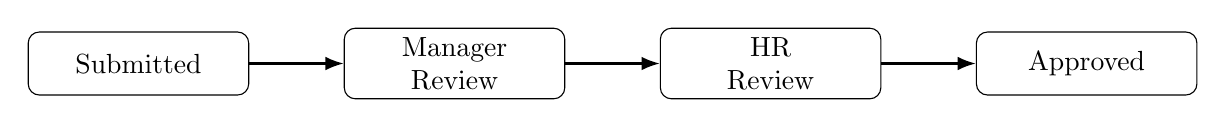
\begin{tikzpicture}[
    node distance=1.2cm,
    box/.style={
        rectangle,
        rounded corners,
        draw,
        align=center,
        minimum width=2.8cm,
        minimum height=0.8cm
    },
    arrow/.style={-{Latex}, thick}
]

\node[box] (submitted) {Submitted};
\node[box, right=of submitted] (manager) {Manager\\Review};
\node[box, right=of manager] (hr) {HR\\Review};
\node[box, right=of hr] (approved) {Approved};

\draw[arrow] (submitted) -- (manager);
\draw[arrow] (manager) -- (hr);
\draw[arrow] (hr) -- (approved);

\end{tikzpicture}
\end{center}

The historical events leading to the final state are retained.

% ============================================================
% 4. PROBLEM STATEMENT
% ============================================================

\section{Problem Statement}

Traditional Human Resource Management Systems (HRMS) primarily
serve as systems of record for maintaining employee information and
processing individual HR transactions. However, conventional
approaches may not provide an integrated representation of the
relationships, dependencies, state transitions, and lifecycle
associated with interconnected HR processes. They may also lack a
controlled mechanism for simulating how a change in one HR process
can affect dependent processes.

The proposed project addresses this requirement by developing an
extensible HR platform that provides:

\begin{itemize}

    \item Maintains a structured and traceable representation of
    employee and HR process states throughout their lifecycle.

    \item Represents key employee lifecycle activities as
    state-driven digital processes with defined transitions and
    outcomes.

    \item Supports configurable, multi-level approval workflows for
    HR applications and organizational processes.

    \item Resolves workflow participants dynamically based on
    organizational relationships, roles, and configured
    permissions.

    \item Maintains an auditable history of significant process
    events, state transitions, and user actions.

    \item Supports controlled downstream state transitions between
    interdependent HR processes.

    \item Provides an extensible architecture through which
    authorized developers can introduce and configure additional
    modules without altering the core workflow and platform
    architecture.

    \item Enforces Role-Based Access Control (RBAC) and the
    principle of least privilege across Developer, HR, Manager, and
    Employee roles.

\end{itemize}


% ============================================================
% 5. OBJECTIVES
% ============================================================

\section{Objectives}

The main objectives of the proposed project are:

\begin{enumerate}

    \item To develop an HRMS that functions as a Process Digital
    Twin of major HR processes.

    \item To maintain an authoritative representation of employees
    and organizational structure.

    \item To support the employee lifecycle from onboarding to
    resignation and exit.

    \item To provide configurable approval workflows for HR
    applications.

    \item To implement Role-Based Access Control for Developer, HR,
    Manager, and Employee roles.

    \item To preserve historical process states and state-changing
    events.

    \item To automatically trigger related HR state changes when
    appropriate.

    \item To provide Employee Self-Service for employee-related
    applications.

    \item To implement a Dynamic Module Engine for future
    extensibility.

    \item To implement dependency validation for dynamically added
    modules.

    \item To model each HR module as a state-driven process with
    defined states, transitions, events, and process dependencies.

    \item To simulate representative HR processes and observe the
    resulting state changes across dependent modules.

    \item To develop a locally runnable prototype using free and
    open-source technologies.

\end{enumerate}

% ============================================================
% 6. HR DIGITAL TWIN MODULES
% ============================================================

\section{HR Digital Twin Modules}

The proposed system incorporates the existing HRMS processes and
introduces additional capabilities to extend the HR Process Digital
Twin.

% ============================================================
% 6.1 PRESENT HRMS MODULES
% ============================================================

\subsection{Present HRMS Modules}

The following modules represent the HR processes currently
available within the organization's HRMS and incorporated into the
proposed Digital Twin.

% ------------------------------------------------------------
\subsubsection{Employee and Document Management}

The Employee and Document Management module maintains the central
employee master and organizational information while managing
HR-related documents associated with employees and HR processes.

The employee management functionality maintains employee identity,
contact details, department, designation, reporting manager,
employment type, joining date, employment status, and relevant
employment history. The employee record acts as a core reference
for other HR processes, avoiding unnecessary duplication of
employee information.

The document management functionality manages authorized HR
documents such as joining documents, certificates, payslips,
supporting documents, declarations, and other employee records.
Relevant document metadata and storage references are maintained
for traceability and controlled access.

Access to employee information and documents is controlled through
Role-Based Access Control according to the responsibilities and
permissions of each user role.

% ------------------------------------------------------------
\subsubsection{Attendance and Leave Management}

The Attendance and Leave Management module records and maintains
employee attendance and leave information. It manages attendance
statuses such as present, absent, late, and half-day, together with
attendance history and authorized corrections.

The module also manages leave types, leave balances, holiday
information, leave applications, approval status, and historical
leave records. Employees can submit leave applications through the
configured approval workflow.

Attendance and leave information can be utilized by other HR
processes such as payroll and Employee Self-Service.

% ------------------------------------------------------------
\subsubsection{Payroll and Statutory Compliance}

The Payroll and Statutory Compliance module manages employee salary
and payroll-related information. It supports salary structures,
earnings, allowances, deductions, gross salary, net salary, payroll
periods, and payslips.

The statutory compliance component maintains configurable records
for Provident Fund (PF), Employee State Insurance (ESI),
Professional Tax, and Tax Deducted at Source (TDS), according to
applicable organizational and regulatory requirements.

The module maintains payroll processing history and provides
authorized employees with access to their applicable payroll
information.

% ------------------------------------------------------------
\subsubsection{Performance and Appraisal Management}

The Performance and Appraisal Management module supports the
systematic evaluation of employee performance and appraisal
outcomes. It manages performance cycles, goals, KPIs, review
periods, manager evaluations, ratings, comments, appraisal
periods, and appraisal outcomes.

The module maintains historical performance and appraisal records
and supports the association of performance results with relevant
employee career processes. Access to evaluation information is
controlled according to organizational roles and permissions.

% ------------------------------------------------------------
\subsubsection{Employee Self-Service (ESS)}

The Employee Self-Service module provides employees with controlled
access to their own HR information and authorized HR services.
Employees can view permitted personal and employment information,
attendance and leave details, payslips, documents, and relevant
employment history.

The module also allows employees to submit authorized HR
applications such as leave, loan, benefits, internal opportunities,
and resignation requests through the configured workflow.

Access is restricted so that employees can access only their own
authorized information and services.

% ------------------------------------------------------------
\subsubsection{Company Asset Management}

The Company Asset Management module maintains records of
organization-owned assets assigned to employees. It records asset
identification, asset type, allocation information, assignment
date, return date, condition, and current status.

The module also supports asset return and clearance as part of
employee exit processing, while maintaining the relevant asset
history.

% ------------------------------------------------------------
\subsubsection{Employee Loan Management}

The Employee Loan Management module enables eligible employees to
submit loan applications through the HRMS. Applications can
contain the requested amount, purpose, supporting documents,
approval status, and relevant repayment information.

Loan applications are processed through the configured workflow,
with approval decisions and processing history maintained for
traceability.

% ------------------------------------------------------------
\subsubsection{Excellence Awards}

The Excellence Awards module supports employee nomination,
recognition, and award processing. It maintains information such as
the nominated employee, award category, reason for nomination,
supporting information, approval status, and award history.

Award nominations can be routed through configurable approval
stages before the recognition is finalized.

% ------------------------------------------------------------
\subsubsection{Special Allowance Management}

The Special Allowance Management module enables eligible employees
to apply for and manage organization-defined allowances and
benefits such as Leave Travel Allowance (LTA), School/Children
Allowance (SCA), and other applicable employee allowances.

The module maintains allowance type, eligibility information,
application details, supporting documents, requested amount,
approval status, and processing history.

Allowance applications are processed through the configured HR
workflow, with appropriate approvals and complete request history
maintained for traceability.

% ============================================================
% 6.2 ADDITIONAL FEATURES
% ============================================================

\subsection{Additional Features}

The following capabilities are introduced as additional features
to extend the existing HRMS and enhance the proposed HR Process
Digital Twin.

% ------------------------------------------------------------
\subsubsection{HR Dashboard}

The HR Dashboard provides a consolidated operational view of
important HR information and pending activities. It can present
summaries such as employee statistics, pending approvals, open
positions, onboarding activities, attendance information, leave
status, and other relevant HR indicators.

The dashboard provides role-appropriate visibility to authorized
users and supports efficient monitoring of HR operations.

% ------------------------------------------------------------
\subsubsection{Recruitment and Candidate Screening}

The Recruitment and Candidate Screening module manages the
recruitment lifecycle from job opening through candidate evaluation
and selection. It maintains job postings, candidate profiles,
applications, resumes, screening status, interview stages, and
selection status.

The module can incorporate AI-assisted resume screening to compare
candidate skills, qualifications, and experience with the
requirements of a job opening. The AI capability is intended to
support HR decision-making and does not independently make
employment decisions.

% ------------------------------------------------------------
\subsubsection{Expense and Reimbursement}

The Expense and Reimbursement module enables employees to submit
eligible business-related expenses for reimbursement. It maintains
expense category, amount, date, description, supporting documents,
approval status, and reimbursement information.

Submitted expenses are processed through the configured approval
workflow before reimbursement is finalized.

% ------------------------------------------------------------
\subsubsection{Rehire and Rejoining Management}

The Rehire and Rejoining Management module manages the process of
bringing a previous employee back into the organization. It
maintains previous employment references, rejoining requests,
eligibility information, approval status, new employment details,
and rejoining history.

The module preserves relevant historical employment information
while establishing the appropriate current employment state after
rejoining.

% ------------------------------------------------------------
\subsubsection{Training and Skills Management}

The Training and Skills Management module manages employee
development activities and skill information. It maintains
training programs, schedules, employee enrolment, completion
status, certifications, skills, skill levels, and skill history.

The module can associate employee skills with organizational
requirements and employee development activities.

% ------------------------------------------------------------
\subsubsection{Notification Management}

The Notification Management module provides a centralized mechanism
for communicating relevant HR events and workflow updates to
authorized users.

Notifications may be generated for events such as new approval
requests, application status changes, leave decisions, job
openings, workflow actions, and other important HR updates.

During employee onboarding, the employee's email address can be
recorded and used for authorized email-based notifications.

% ------------------------------------------------------------
\subsubsection{Shift Management}

The Shift Management module manages employee work-shift
assignments. It maintains shift definitions, working hours, shift
assignments, effective dates, and employee-wise shift information.

The module can be integrated with Attendance and Leave Management
so that attendance records can be interpreted according to the
employee's assigned shift.

% ------------------------------------------------------------
\subsubsection{Project Management}

The Project Management module manages the association of employees
with organizational projects and project activities. It maintains
project information, project members, employee assignments, project
roles, project status, tasks, and project timelines.

The module provides an organizational view of employee involvement
across projects while maintaining appropriate access control.

% ------------------------------------------------------------
\subsubsection{Promotion and Transfer Management}

The Promotion and Transfer Management module manages employee
career movement within the organization.

\textbf{Promotion} represents the movement of an employee to a
higher designation or position based on organizational requirements,
eligibility, performance, and approval.

\textbf{Internal Transfer} represents the movement of an existing
employee from one department, organizational unit, designation, or
location to another.

Both processes are handled through configurable workflows and
maintain relevant historical employment information. Required
organizational changes are applied only after the configured
approval stages are completed.

For example, an internal transfer may follow:

\[
\begin{array}{c}
\text{Transfer Request} \\[4pt]
\downarrow \\[4pt]
\text{Current Manager Review} \\[4pt]
\downarrow \\[4pt]
\text{HR Review} \\[4pt]
\downarrow \\[4pt]
\text{New Manager Review} \\[4pt]
\downarrow \\[4pt]
\text{Approval} \\[4pt]
\downarrow \\[4pt]
\text{Effective Transfer}
\end{array}
\]

The employee's organizational and relevant employment history are
updated only after the required approvals are completed.
% ------------------------------------------------------------

% ------------------------------------------------------------
\subsubsection{Module Process Simulation and Dependencies}

Each HR module in the proposed Digital Twin is represented as a
state-driven process with defined inputs, states, transitions,
events, and dependencies. A common simulation mechanism is used so
that the behaviour of different modules can be executed and observed
without creating a separate simulation engine for each module.

Representative process dependencies include:

\begin{itemize}
    \item Attendance and Leave Management $\rightarrow$ Payroll and
    Statutory Compliance
    \item Performance and Appraisal Management $\rightarrow$
    Promotion and Transfer Management
    \item Resignation and Exit $\rightarrow$ Position Vacancy $\rightarrow$
    Promotion or Recruitment
    \item Shift Management $\rightarrow$ Attendance and Leave
    Management
    \item Training and Skills Management $\rightarrow$ Performance and
    Appraisal / Promotion processes
    \item Recruitment and Candidate Screening $\rightarrow$
    Employee and Document Management / Onboarding
    \item Expense and Reimbursement $\rightarrow$ Payroll and
    Statutory Compliance, where applicable
\end{itemize}

During simulation, a state-changing event in one module is evaluated
against its configured dependencies. Where a dependency condition is
satisfied, the corresponding downstream process state or event is
updated and recorded. This provides a controlled representation of
how interconnected HR processes behave across the Digital Twin.

% 6.3 CORE PLATFORM AND DIGITAL TWIN CAPABILITIES
% ============================================================

\subsection{Core Platform and Digital Twin Capabilities}

The proposed HR Process Digital Twin is supported by a set of
common platform capabilities that provide workflow control,
extensibility, process-state management, and traceability across
the HRMS. These capabilities operate across multiple HR modules
rather than functioning as independent HR business modules.

% ------------------------------------------------------------
\subsubsection{Application and Workflow Management}

The Application and Workflow Management capability provides a
standardized mechanism for submitting, processing, approving, and
tracking HR applications and organizational requests.

It supports configurable workflow stages, role-based approval,
application status management, comments, attachments, and
workflow history. Approvers can be resolved dynamically based on
organizational relationships, reporting structures, and configured
permissions rather than being permanently assigned within the
application logic.

The same workflow mechanism can be reused across different HR
processes such as leave applications, employee loans, expense
claims, promotion, transfer, and resignation.

% ------------------------------------------------------------
\subsubsection{Dynamic Module and Dependency Management}

The Dynamic Module and Dependency Management capability provides
an extensible architecture for introducing additional HR
functionality without modifying the core platform.

Authorized developers can register and configure new modules with
information such as module identity, version, permissions,
workflow requirements, and dependencies.

Before a module is activated, its required dependencies are
validated to ensure that the required modules and compatible
versions are available. Circular or unresolved dependencies are
identified and module activation is prevented until the dependency
requirements are satisfied.

This approach allows the HRMS to evolve as organizational
requirements change while maintaining controlled module
configuration.

% ------------------------------------------------------------
\subsubsection{Digital Twin State and Event Management}

The Digital Twin State and Event Management capability maintains
the current state of important HR entities and processes while
recording the events responsible for state transitions.

For example, an employee resignation process can progress through
the following states:

\[
\begin{array}{c}
\text{Active Employee} \\[3pt]
\downarrow \\[3pt]
\text{Resignation Submitted} \\[3pt]
\downarrow \\[3pt]
\text{Under Review} \\[3pt]
\downarrow \\[3pt]
\text{Approved} \\[3pt]
\downarrow \\[3pt]
\text{Exiting} \\[3pt]
\downarrow \\[3pt]
\text{Exited}
\end{array}
\]

Each significant state transition generates a corresponding event
containing relevant information such as the event type, affected
entity, initiating user, timestamp, and resulting state.

Maintaining the current state together with the historical event
record provides a traceable digital representation of the HR
process lifecycle. During simulation, these states and events are
used to reproduce defined process transitions and evaluate their
configured dependencies. This state-and-event representation forms a
core component of the proposed HR Process Digital Twin.
% ------------------------------------------------------------
\subsubsection{Audit and Traceability}

The Audit and Traceability capability maintains records of
significant actions and state-changing operations performed within
the HRMS.

Audit information can include:

\begin{itemize}

    \item User who performed the action

    \item User role

    \item Action performed

    \item Affected entity and entity identifier

    \item Previous state or value, where applicable

    \item New state or value, where applicable

    \item Date and time of the operation

    \item Relevant comments or reason

\end{itemize}

The audit mechanism provides accountability and traceability for
HR operations and allows authorized users to determine how and
when significant changes occurred within an HR process.
% ============================================================
% 7. APPLICATION AND REQUEST ENGINE
% ============================================================

\section{Application and Request Engine}

The Application and Request Engine provides one reusable mechanism
for employee requests.

Instead of implementing separate application logic for every HR
module, requests such as leave, loan, promotion, transfer and
resignation use a common Application entity.

Each application contains:

\begin{itemize}
    \item Application ID
    \item Employee
    \item Application type
    \item Module
    \item Submission date
    \item Current status
    \item Current workflow step
    \item Final decision
    \item Comments
    \item Attachments
    \item Timestamps
\end{itemize}

Adding a new request type should be configuration-driven instead of
requiring a new hard-coded request architecture.
% ============================================================
% 8. KEY END-TO-END WORKFLOW
% ============================================================

\section{Key End-to-End Workflow: Resignation to Vacancy}

A key demonstration of the proposed HR Process Digital Twin is the
relationship between employee resignation and the resulting
organizational position state.

The process can be represented as:

\begin{center}
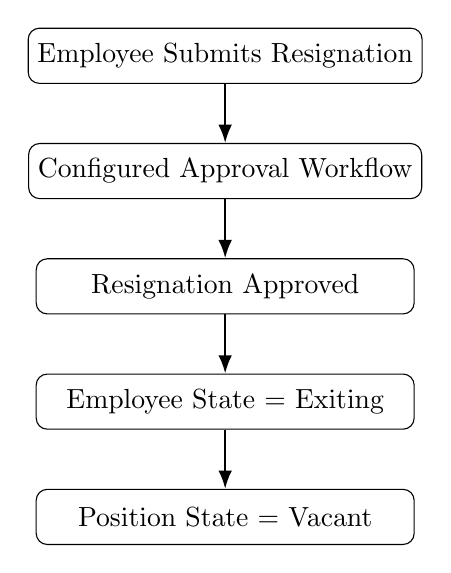
\begin{tikzpicture}[
    node distance=0.75cm,
    box/.style={
        rectangle,
        rounded corners,
        draw,
        align=center,
        minimum width=4.8cm,
        minimum height=0.7cm
    },
    arrow/.style={-{Latex}, thick}
]

\node[box] (resign) {Employee Submits Resignation};
\node[box, below=of resign] (review) {Configured Approval Workflow};
\node[box, below=of review] (approved) {Resignation Approved};
\node[box, below=of approved] (exiting) {Employee State = Exiting};
\node[box, below=of exiting] (vacant) {Position State = Vacant};

\draw[arrow] (resign) -- (review);
\draw[arrow] (review) -- (approved);
\draw[arrow] (approved) -- (exiting);
\draw[arrow] (exiting) -- (vacant);

\end{tikzpicture}
\end{center}

Once the position becomes vacant, the system can make the vacancy
available for the configured organizational process. Where
applicable, an eligible internal employee may be considered through
the Promotion and Transfer workflow. If an internal candidate is
not selected, the position can proceed through the configured
recruitment or job requisition process.

The system maintains the state transitions and associated events,
providing traceability from the employee's resignation to the
resulting position state.

The system does not automatically promote or select an employee;
such decisions remain subject to the configured approval workflow
and authorized users.
% ============================================================
% 9. ROLE BASED ACCESS
% ============================================================

\section{Role-Based Access Control}

The system follows least-privilege access.

\begin{center}
\begin{longtable}{@{}p{3cm}p{9cm}@{}}
\toprule
\textbf{Role} & \textbf{Primary Responsibilities} \\
\midrule

Developer &
Register and manage modules, dependencies, permissions,
workflow definitions, module versions and technical health.
Does not receive default access to confidential HR data. \\

HR &
Organization-wide HR operations including employees, onboarding,
requisitions, vacancies, payroll, benefits, promotions, transfers,
resignations, documents and assets. \\

Manager &
Assigned team management including leave approvals, performance
evaluation, promotion recommendations, transfer/resignation review,
and job requisitions. \\

Employee &
Own profile, attendance, leave, payslips, benefits, documents,
applications, internal vacancies, promotion/transfer history and
resignation. \\

\bottomrule
\end{longtable}
\end{center}

\subsection{Access Rules}

\begin{itemize}
    \item Employees can access only their own confidential data.
    \item Managers can access only their authorized teams.
    \item HR can manage organization-wide HR operations.
    \item Developers can manage platform configuration but do not
    automatically gain confidential HR access.
\end{itemize}

% ============================================================
% 10. PROPOSED SYSTEM ARCHITECTURE
% ============================================================

\section{Proposed System Architecture}

The proposed HR Process Digital Twin follows a
\textbf{modular monolith architecture}. The architecture is
organized into presentation, application and security, HR business
modules, core Digital Twin and simulation capabilities, and data
persistence layers. The design provides a common platform for
existing HRMS processes while allowing additional modules and their
process dependencies to be introduced in a controlled and extensible
manner.

\subsection{High-Level Architecture}

\begin{center}

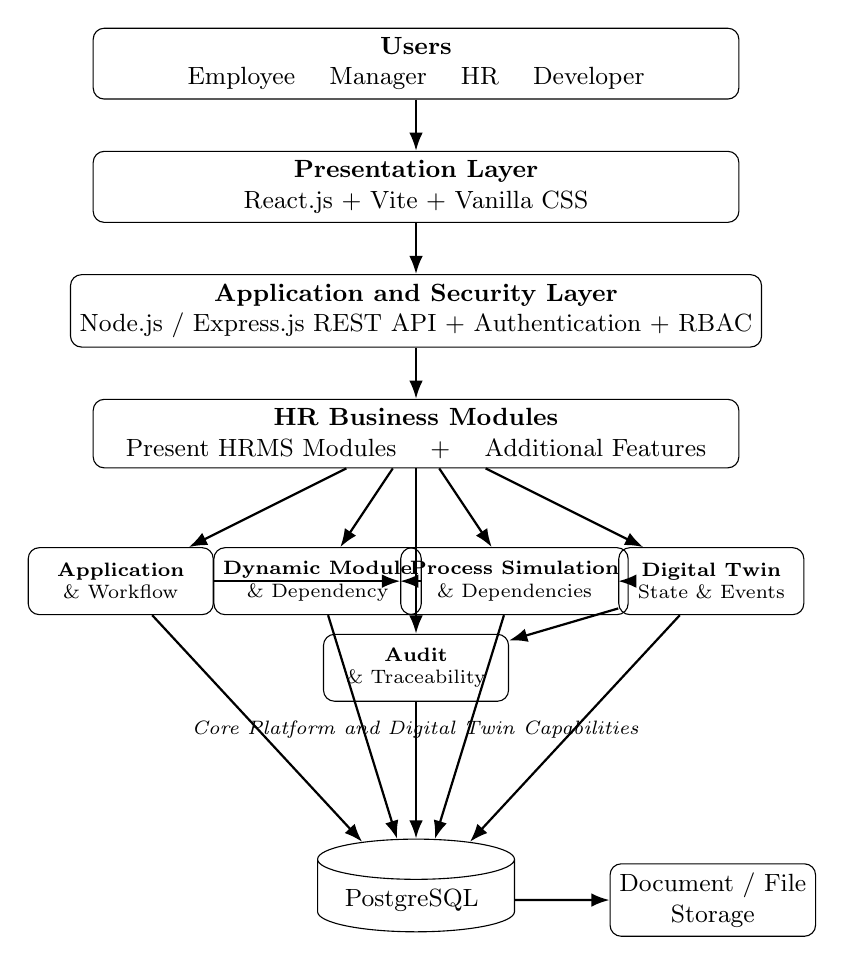
\begin{tikzpicture}[
    node distance=0.65cm,
    layer/.style={
        rectangle,
        rounded corners,
        draw,
        align=center,
        minimum width=8.2cm,
        minimum height=0.75cm,
        font=\small
    },
    capability/.style={
        rectangle,
        rounded corners,
        draw,
        align=center,
        minimum width=2.35cm,
        minimum height=0.85cm,
        font=\scriptsize
    },
    database/.style={
        cylinder,
        shape border rotate=90,
        aspect=0.25,
        draw,
        align=center,
        minimum width=2.5cm,
        minimum height=0.9cm,
        font=\small
    },
    storage/.style={
        rectangle,
        rounded corners,
        draw,
        align=center,
        minimum width=2.5cm,
        minimum height=0.75cm,
        font=\small
    },
    arrow/.style={
        -{Latex},
        thick
    }
]

% ============================================================
% USERS
% ============================================================

\node[layer] (users)
{
\textbf{Users}\\
Employee \quad Manager \quad HR \quad Developer
};

% ============================================================
% PRESENTATION
% ============================================================

\node[layer, below=of users] (presentation)
{
\textbf{Presentation Layer}\\
React.js + Vite + Vanilla CSS
};

% ============================================================
% API + SECURITY
% ============================================================

\node[layer, below=of presentation] (api)
{
\textbf{Application and Security Layer}\\
Node.js / Express.js REST API + Authentication + RBAC
};

% ============================================================
% HR BUSINESS MODULES
% ============================================================

\node[layer, below=of api] (hrmodules)
{
\textbf{HR Business Modules}\\
Present HRMS Modules \quad + \quad Additional Features
};

% ============================================================
% CORE CAPABILITIES
% ============================================================

\node[capability, below=1cm of hrmodules,
      xshift=-3.75cm] (workflow)
{
\textbf{Application}\\
\& Workflow
};

\node[capability, below=1cm of hrmodules,
      xshift=-1.25cm] (dynamic)
{
\textbf{Dynamic Module}\\
\& Dependency
};

\node[capability, below=1cm of hrmodules,
      xshift=1.25cm] (simulation)
{
\textbf{Process Simulation}\\
\& Dependencies
};

\node[capability, below=1cm of hrmodules,
      xshift=3.75cm] (twin)
{
\textbf{Digital Twin}\\
State \& Events
};

\node[capability, below=2.1cm of hrmodules,
      xshift=0cm] (audit)
{
\textbf{Audit}\\
\& Traceability
};

% ============================================================
% COMMON PLATFORM LABEL
% ============================================================

\node[font=\scriptsize, below=0.12cm of audit.south] (platform)
{
\textit{Core Platform and Digital Twin Capabilities}
};

% ============================================================
% DATA PERSISTENCE
% ============================================================

\node[database, below=1.15cm of platform] (database)
{
PostgreSQL
};

\node[storage, right=1.2cm of database] (storage)
{
Document / File\\
Storage
};

% ============================================================
% CONNECTIONS
% ============================================================

\draw[arrow] (users) -- (presentation);
\draw[arrow] (presentation) -- (api);
\draw[arrow] (api) -- (hrmodules);

\draw[arrow] (hrmodules) -- (workflow);
\draw[arrow] (hrmodules) -- (dynamic);
\draw[arrow] (hrmodules) -- (simulation);
\draw[arrow] (hrmodules) -- (twin);
\draw[arrow] (hrmodules) -- (audit);

\draw[arrow] (workflow) -- (simulation);
\draw[arrow] (dynamic) -- (simulation);
\draw[arrow] (simulation) -- (twin);
\draw[arrow] (twin) -- (audit);
\draw[arrow] (workflow) -- (database);
\draw[arrow] (dynamic) -- (database);
\draw[arrow] (simulation) -- (database);
\draw[arrow] (twin) -- (database);
\draw[arrow] (audit) -- (database);

\draw[arrow] (database) -- (storage);

\end{tikzpicture}

\end{center}

\subsection{Architecture Components}

\begin{itemize}

    \item \textbf{Users:}
    The system provides role-specific access for Employee, Manager,
    HR, and Developer users.

    \item \textbf{Presentation Layer:}
    Provides the web interface using React.js, Vite, and
    Vanilla CSS.

    \item \textbf{Application and Security Layer:}
    Node.js and Express.js provide the REST API and application interface, while
    authentication and Role-Based Access Control restrict access
    according to the user's role and permissions.

    \item \textbf{HR Business Modules:}
    Contains the existing HRMS modules and the additional features
    implemented within the proposed system.

    \item \textbf{Application and Workflow Management:}
    Provides reusable application processing and configurable
    approval workflows with dynamically resolved approvers.

    \item \textbf{Dynamic Module and Dependency Management:}
    Allows authorized developers to introduce new modules and
    validates their registered dependencies before activation.

    \item \textbf{Process Simulation and Dependency Management:}
    Represents module-level process states, transitions, and
    dependencies and supports controlled simulation of downstream
    state changes between interconnected HR processes.

    \item \textbf{Digital Twin State and Event Management:}
    Maintains the current state of important HR processes and
    preserves the events associated with significant state
    transitions.

    \item \textbf{Audit and Traceability:}
    Records significant state-changing operations to provide
    accountability and historical traceability.

    \item \textbf{Data Persistence:}
    PostgreSQL stores structured HRMS, workflow, module, Digital
    Twin, and audit data, while document and file storage maintains
    uploaded HR documents.

\end{itemize}
% ============================================================
% 11. DATA REQUIREMENTS
% ============================================================

\section{Data Requirements}

The proposed HR Process Digital Twin requires structured data to
represent employees, organizational relationships, HR transactions,
workflow processes, and the current and historical state of HR
operations.

\subsection{Identity and Access Data}

The system maintains user accounts, roles, permissions, and session
information required for authentication and Role-Based Access
Control.

\subsection{Employee and Organization Data}

The system maintains employee profiles, employment history,
departments, designations, organizational units, positions, and
reporting relationships. This information forms the foundation for
employee-related HR processes and dynamic approver resolution.

\subsection{HR Transaction Data}

The system maintains operational HR information including
attendance, leave, performance, appraisal, payroll, statutory
records, employee loans, benefits, awards, and company asset
assignments.

\subsection{Recruitment and Career Data}

The system maintains job requisitions, job openings, candidate
information, recruitment status, promotions, internal transfers,
resignations, and employee exit information.

\subsection{Application and Workflow Data}

The system maintains HR applications and their associated workflow
information, including application type, current status, workflow
stage, approvers, approval decisions, comments, attachments, and
processing history.

\subsection{Document Data}

The system maintains document metadata and references associated
with employees and HR transactions. Uploaded documents may include
joining documents, certificates, supporting documents, and other
authorized HR records.

\subsection{Digital Twin and Audit Data}

The Digital Twin maintains the current state of relevant HR
entities and processes together with the historical events
associated with state transitions.

The system also maintains audit information such as the user,
action, affected entity, timestamp, previous state, and resulting
state where applicable. This enables traceability of significant
HR operations.

\subsection{Process Simulation Data}

The Digital Twin maintains process definitions, states, state
transitions, process events, dependency relationships, dependency
conditions, and simulation scenario data required to represent and
execute controlled HR process simulations.

\subsection{Module and Dependency Data}

The platform maintains information about registered modules,
versions, dependencies, permissions, and activation status. This
information enables authorized developers to introduce additional
modules while ensuring that their required dependencies are
available.

The \textbf{Employee} entity is treated as a core entity within the
system. Other HR modules reference the employee through its unique
identifier rather than duplicating employee information. This
provides consistency and establishes relationships between the
employee and different HR processes throughout the Digital Twin.

% ============================================================
% 12. DATABASE DESIGN
% ============================================================

\section{Database Design}

PostgreSQL is used as the primary relational database for storing
structured HRMS and Digital Twin data. The database follows a
normalized relational structure with appropriate primary keys,
foreign-key relationships, constraints, indexes, and timestamps.

The database is designed around the Employee entity, which acts as
a central reference for multiple HR processes. Other modules
associate their records with the employee through a unique
\texttt{employee\_id} rather than duplicating employee information.

\subsection{Core Entity Relationships}

The major relationships between the employee and selected HR
processes can be represented as follows:

\begin{center}

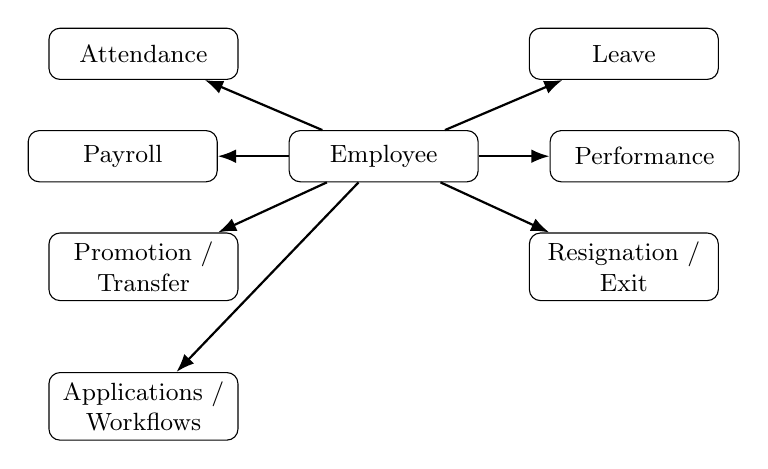
\begin{tikzpicture}[
    node distance=0.9cm,
    entity/.style={
        rectangle,
        rounded corners,
        draw,
        align=center,
        minimum width=2.4cm,
        minimum height=0.65cm,
        font=\small
    },
    arrow/.style={-{Latex}, thick}
]

\node[entity] (employee) {Employee};

\node[entity, above left=of employee] (attendance)
    {Attendance};

\node[entity, above right=of employee] (leave)
    {Leave};

\node[entity, left=of employee] (payroll)
    {Payroll};

\node[entity, right=of employee] (performance)
    {Performance};

\node[entity, below left=of employee] (career)
    {Promotion /\\Transfer};

\node[entity, below right=of employee] (exit)
    {Resignation /\\Exit};

\node[entity, below=of career] (application)
    {Applications /\\Workflows};

\draw[arrow] (employee) -- (attendance);
\draw[arrow] (employee) -- (leave);
\draw[arrow] (employee) -- (payroll);
\draw[arrow] (employee) -- (performance);
\draw[arrow] (employee) -- (career);
\draw[arrow] (employee) -- (exit);
\draw[arrow] (employee) -- (application);

\end{tikzpicture}

\end{center}

In addition to employee-related records, the database maintains
organizational information, user roles and permissions, documents,
assets, benefits, recruitment information, module configuration,
workflow definitions, Digital Twin states and events, and audit
records.

The database also supports the process simulation model by storing
process states, transitions, dependency relationships, simulation
scenario data, and generated events. These records allow the system
to reproduce configured HR process behaviour and maintain the
resulting state history.

The database therefore provides the persistent data layer for both
the existing HRMS processes and the additional capabilities of the
proposed HR Process Digital Twin.

% ============================================================
% 13. TECHNOLOGY STACK
% ============================================================

\section{Technology Stack}

The proposed system uses a modern open-source technology stack
suitable for developing and locally deploying the HR Process Digital
Twin.

\begin{center}
\begin{longtable}{@{}p{4cm}p{8.5cm}@{}}
\toprule
\textbf{Layer} & \textbf{Technology} \\
\midrule

Frontend &
React.js, Vite, Vanilla CSS \\

Backend &
Node.js, Express.js, PostgreSQL Driver (pg) \\

Database &
PostgreSQL \\

\bottomrule
\end{longtable}
\end{center}

\subsection{Frontend}

React.js is used to develop the role-specific user
interfaces for Employee, Manager, HR, and Developer roles. Vite
provides the frontend development and build environment, while
Vanilla CSS is used for the user interface styling.

\subsection{Backend}

Node.js with Express.js provides the application and REST API layer.
The \texttt{pg} (node-postgres) module provides the database interaction
layer, allowing secure execution of parameterized SQL queries.

\subsection{Database}

PostgreSQL is used as the primary relational database for storing
employee information, organizational data, HR transactions,
applications, workflows, module configuration, Digital Twin states,
events, and audit records.

\subsection{Authentication and Security}

The system uses Employee ID and password as the primary login
mechanism. Passwords are securely hashed using Argon2id, while
HTTP-only cookies and Role-Based Access Control are used to protect
authenticated sessions and restrict access according to user roles.

\subsection{Real-Time Communication}

React state management and API polling are used where required to provide real-time
updates for Digital Twin state changes, workflow notifications, and
other relevant system events.

\subsection{File Storage}
Document metadata and storage references are maintained
in PostgreSQL.
% ============================================================
% 14. NON-FUNCTIONAL REQUIREMENTS
% ============================================================

\section{Non-Functional Requirements}

\subsection{Security}

The system will provide:

\begin{itemize}
    \item Argon2id password hashing
    \item HTTP-only secure cookies
    \item RBAC and permission checks
    \item Input validation
    \item Environment-based secrets
    \item No sensitive data in logs
\end{itemize}

\subsection{Auditability}

Every state-changing operation will maintain:

\begin{itemize}
    \item User
    \item Role
    \item Action
    \item Entity
    \item Entity ID
    \item Relevant old/new values
    \item Timestamp
    \item Comments
\end{itemize}

\subsection{Extensibility}

New modules should be addable without modifying the core Workflow
Engine or Module Engine.

\subsection{Data Integrity}

The database will use:

\begin{itemize}
    \item Foreign keys
    \item Constraints
    \item Indexes
    \item Timestamps
    \item Normalized relational structures
\end{itemize}


% ============================================================
% 15. VALIDATION AND TESTING
% ============================================================

\section{Validation and Testing}

The proposed system will be validated through functional,
security, workflow, module, and Digital Twin state testing.

\subsection{Authentication and Access Testing}

The system will verify that:

\begin{itemize}
    \item Valid Employee ID and password allow authentication.
    \item Invalid credentials are rejected.
    \item Inactive accounts cannot authenticate.
    \item Users can access only the information and operations
    permitted by their assigned role.
\end{itemize}

\subsection{Workflow Testing}

The system will verify that:

\begin{itemize}
    \item Applications follow their configured approval workflow.
    \item Unauthorized users cannot perform approval actions.
    \item Approvers are resolved according to organizational
    relationships and permissions.
    \item Approved and rejected requests reach the appropriate
    process state.
    \item Workflow history is preserved.
\end{itemize}

\subsection{Module and Dependency Testing}

The system will verify that:

\begin{itemize}
    \item Authorized developers can register new modules.
    \item Required dependencies are correctly identified.
    \item Missing or inactive dependencies prevent activation.
    \item Incompatible dependencies are detected.
    \item Successfully validated modules can be activated.
\end{itemize}

\subsection{Digital Twin State Testing}

The system will verify that significant HR events correctly update
the corresponding Digital Twin state.

For example:

\[
\text{Resignation Approved}
\rightarrow
\text{Employee State = Exiting}
\]

The system will also verify that the historical event remains
available after the state transition, thereby maintaining
traceability of the HR process lifecycle.
\subsection{Process Simulation and Dependency Testing}

The system will verify that each configured HR process can be
simulated through its defined states and transitions and that
configured dependencies produce the expected downstream effects.

Representative scenarios include:

\begin{itemize}
    \item Approved leave updating the corresponding attendance and
    leave states and providing relevant input to payroll processing.
    \item Completed performance and appraisal processes providing
    relevant input to promotion-related processing.
    \item Approved resignation changing the employee state and
    resulting in a position vacancy.
    \item A vacant position becoming available to the configured
    promotion or recruitment process.
    \item Shift assignments affecting the interpretation of attendance
    records.
\end{itemize}

The expected state transitions, dependency conditions, and generated
events will be compared with the configured simulation results.

% ============================================================
% 21. DEMO / ACCEPTANCE SCENARIOS
% ============================================================

\section{Demo and Acceptance Scenarios}

The Phase 1 prototype should demonstrate the following scenarios:

\begin{enumerate}

    \item Employee logs into the system and accesses only the
    information permitted by the assigned role.

    \item Leave approval is simulated and the resulting attendance
    and payroll-related dependency states are displayed.

    \item Performance and appraisal completion is simulated and the
    resulting promotion-related process dependency is displayed.

    \item Resignation approval is simulated, changing the employee
    state to exiting and the corresponding position state to vacant.

    \item The vacant position is evaluated against the configured
    promotion or recruitment dependency.

    \item Shift assignment is simulated and its dependency on
    attendance interpretation is displayed.

    \item A future module is registered and its module dependencies
    are validated before activation.

    \item The Digital Twin displays the current process states,
    generated events, dependency transitions, and historical records
    produced during simulation.

\end{enumerate}

% ============================================================
% 16. EXPECTED RESULTS
% ============================================================

\section{Expected Results}

The proposed system is expected to provide the following outcomes:

\begin{itemize}

    \item A functional Human Resource Management System based on
    the Process Digital Twin approach.

    \item A digital representation of the current and historical
    states of important HR processes.

    \item Integrated management of employee lifecycle processes
    from onboarding through employment and exit.

    \item Secure Employee-Id-based authentication and
    role-based access control for Employee, Manager, HR, and
    Developer roles.

    \item Configurable HR application and approval workflows with
    dynamic approver resolution.

    \item Traceable state transitions and historical event records
    for important HR processes.

    \item Support for the organization's existing HRMS processes
    together with the proposed additional HR capabilities.

    \item Controlled promotion, internal transfer, resignation,
    and related employee lifecycle workflows.

    \item Dynamic module registration and dependency-aware
    activation for future extensibility.

    \item Auditability of significant HR operations and
    state-changing actions.

    \item Controlled simulation of HR modules using configurable
    process states, transitions, events, and dependencies.

    \item Representation and observation of downstream state changes
    between interconnected HR modules.

    \item A locally deployable and cost-efficient prototype using
    open-source technologies.

\end{itemize}

% ============================================================
% 17. LIMITATIONS
% ============================================================

\section{Limitations}

The initial implementation of the proposed HR Process Digital Twin
has the following limitations:

\begin{itemize}

    \item Official confidential company HR data is not provided for
    development. Therefore, sample and configurable data will be
    used for the prototype.

    \item Company-specific HR policies, business rules, and
    organizational configurations will not be assumed unless
    explicitly provided.

    \item The system is initially designed for local deployment and
    does not depend on AWS or other paid cloud services.

    \item The accuracy of configurable HR workflows and approval
    rules depends on the organizational information and policies
    provided during system configuration.

    \item AI-powered resume screening will be treated as an
    assisted decision-support capability and will not make
    autonomous recruitment or employment decisions.

    \item Process simulation uses configurable sample data and
    defined business rules rather than complete real-time enterprise
    data.

    \item External enterprise integrations such as biometric
    attendance devices, enterprise identity providers, payroll
    gateways, and other third-party systems are outside the initial
    prototype scope.

    \item Advanced predictive HR analytics and large-scale
    workforce forecasting are outside the initial prototype scope.

    \item The initial implementation uses local file storage for
    uploaded HR documents rather than enterprise cloud document
    storage.

    \item The system is intended as a prototype representation of
    HR processes and does not replace the organization's official
    HRMS or statutory systems.

\end{itemize}

% ============================================================
% 18. CONCLUSION
% ============================================================

\section{Conclusion}

The proposed project presents a human resource management system based on a process digital twin approach. The system goes beyond conventional HR record management by digitally representing HR processes, their current states, participating users, approval stages, events, and historical changes.

The proposed system represents the organisation's existing HRMS
processes, including employee management, attendance, leave, payroll
and statutory compliance, performance management, Employee
Self-Service, document management, company asset management,
appraisal, employee loans, excellence awards, and special allowances.
It also introduces additional capabilities including an HR
dashboard, AI-powered resume screening, expense and reimbursement,
rehire management, training and skills management, notification
management, shift management, recruitment management, project
management, and promotion and transfer management.

The application and workflow management capability provides
configurable approval processes and dynamically resolves
authorized approvers based on organizational relationships, roles,
and permissions. This allows common workflow mechanisms to be
reused across different HR processes without hard-coding individual
approval chains.

The Dynamic Module and Dependency Management capability provides
extensibility by allowing authorized developers to introduce and
configure additional modules. Registered dependencies are
validated before module activation, helping maintain controlled
and consistent module integration.

The Digital Twin State and Event Management capability maintains
the current state of important HR processes while preserving their
historical events. Combined with process simulation and dependency
management, it enables interconnected HR processes to be simulated,
allowing downstream state changes such as resignation, position
vacancy, and subsequent promotion or recruitment activities to be
represented and traced digitally.

The proposed technology stack of React.js, Vite, Node.js, Express.js,
and PostgreSQL provides a practical and cost-efficient
foundation for implementation. The system is designed to support
local deployment without dependence on AWS or other paid cloud
services.

Overall, the project provides an extensible foundation for
digitally representing, managing, simulating, and tracing
interconnected HR processes as a Process Digital Twin while allowing
the platform to evolve through controlled addition of new modules
and future enterprise integrations.

% ============================================================
% REFERENCES
% ============================================================

\newpage

\section{References}

\begin{enumerate}

    \item Grieves, M., and Vickers, J.,
    ``Digital Twin: Mitigating Unpredictable, Undesirable Emergent
    Behavior in Complex Systems,'' in
    \textit{Transdisciplinary Perspectives on Complex Systems},
    Springer, 2017.

    \item Tao, F., Zhang, H., Liu, A., and Nee, A. Y. C.,
    ``Digital Twin in Industry: State-of-the-Art,''
    \textit{IEEE Transactions on Industrial Informatics},
    vol. 15, no. 4, pp. 2405--2415, 2019.

    \item International Organization for Standardization,
    \textit{ISO 23247: Automation systems and integration --
    Digital twin framework for manufacturing},
    ISO, 2021.

    \item Node.js Documentation,
    ``Node.js: JavaScript runtime built on Chrome's V8 JavaScript engine,''
    Node.js Foundation.

    \item Express.js Documentation,
    ``Express: Fast, unopinionated, minimalist web framework for Node.js,''
    OpenJS Foundation.

    \item PostgreSQL Documentation,
    ``PostgreSQL: The World's Most Advanced Open Source Relational
    Database,'' PostgreSQL Documentation.

    \item Node-Postgres Documentation,
    ``pg: Non-blocking PostgreSQL client for Node.js,''
    Node-Postgres.

    \item React Documentation,
    ``React: The Library for Web and Native User Interfaces,''
    React Documentation.

\end{enumerate}

% ============================================================
% END
% ============================================================

\end{document}
